\subsection{Related Works}
\label{sec:swapping_related}

There have been a few works in the recent years that have addressed generating long-distance \epss
efficiently. All of these works have focused on selecting an efficient routing path~\cite{sigcomm20,yiming2023,yuhang2023} for the swapping
process (Callefi~\cite{caleffi} also selects a path, but using a metric based
on balanced trees).
In addition, all except~\cite{caleffi} have looked at the \os protocol of generating the
\epss. Recall that in the \os model, selection of paths suffice, while in the \wt model, one needs
to consider selection of efficient swapping trees with high fidelity.
%%%%%%%%%%%%%%%%%%%%%%%
Selection of optimal swapping trees is a fundamentally more challenging problem 
than selection of paths---and has not 
been addressed before, to the best of our knowledge. \eat{Efficient use of intermediate \epss rather than
discarding them (as in the \os protocol) has been mentioned as an open problem in~\cite{sigcomm20};
our paper addresses this challenge by using the \wt protocol.} We start with discussing how the \os model
works.

\para{\os Approaches.}
The most recent works to address the above problem are~\cite{sigcomm20} and~\cite{delft-lp}, 
both of which consider the \os model. 
In particular, Shi and Qian~\cite{sigcomm20} design a Dijkstra-like algorithm to construct an optimal path
between a pair of nodes, when there are multiple links (channels) between adjacent nodes. Then,
they use the algorithm iteratively to select multiple paths over multiple pairs of nodes.
~\cite{yuhang2023} is an improvement of~\cite{sigcomm20} that proposes a synchronous multi-time-slot entanglement routing framework
based on the idea of reusing the established but unused EP pairs in subsequent time slots.
Chakraborty et al.~\cite{delft-lp} design a multi-commodity-flow
like LP formulation to select routing paths for a set of source destination pairs. They map
the operation-based fidelity constraint to the path length (as in~\cite{BreigelEtAl1998}), and use
node copies to model the constraint in the LP. However, they explicitly assume that the link
\eps generation is deterministic---i.e., always succeeds. 
%%%%%%%%%%%%%%%%%%%%%%%%%%%%%%%%%%%%%
Among earlier relevant works,~\cite{guha} proposes a greedy solution
for grid networks, and~\cite{greedy2019distributed} proposes 
virtual-path based routing in ring/grid networks.
\eat{and~\cite{gradient} using a gradient approach to select
efficient routing paths.}

\para{\wt Approach.}
Due to photon loss, establishing long-distance entanglement between remote
nodes at $L$ distance by \textit{direct} 
transmission yields \eps rates that decay exponentially with $L$. 
DLCZ protocol~\cite{dlcz,gisin} broke this exponential barrier using
$2^k$ equidistant intermediate nodes to perform entanglement-swapping operations, 
implicitly over a balanced binary tree, with a \wt protocol; this makes the 
\eps generation rate decay only polynomially in $L$. \eat{This is fundamental to the feasibility of establishing long-distance entanglements.}
%%%%%%%%%%%%
More recently, Caleffi~\cite{caleffi} formulated the entanglement generation rate on a given path between two nodes, under the more realistic condition where the intermediate nodes in the path may not all be equidistant, but still considered only balanced trees. Their path-based metric
%%%%%
was then used to select the optimal path by enumerating over the 
exponentially many paths in the network.

\begin{figure}
    \centering
    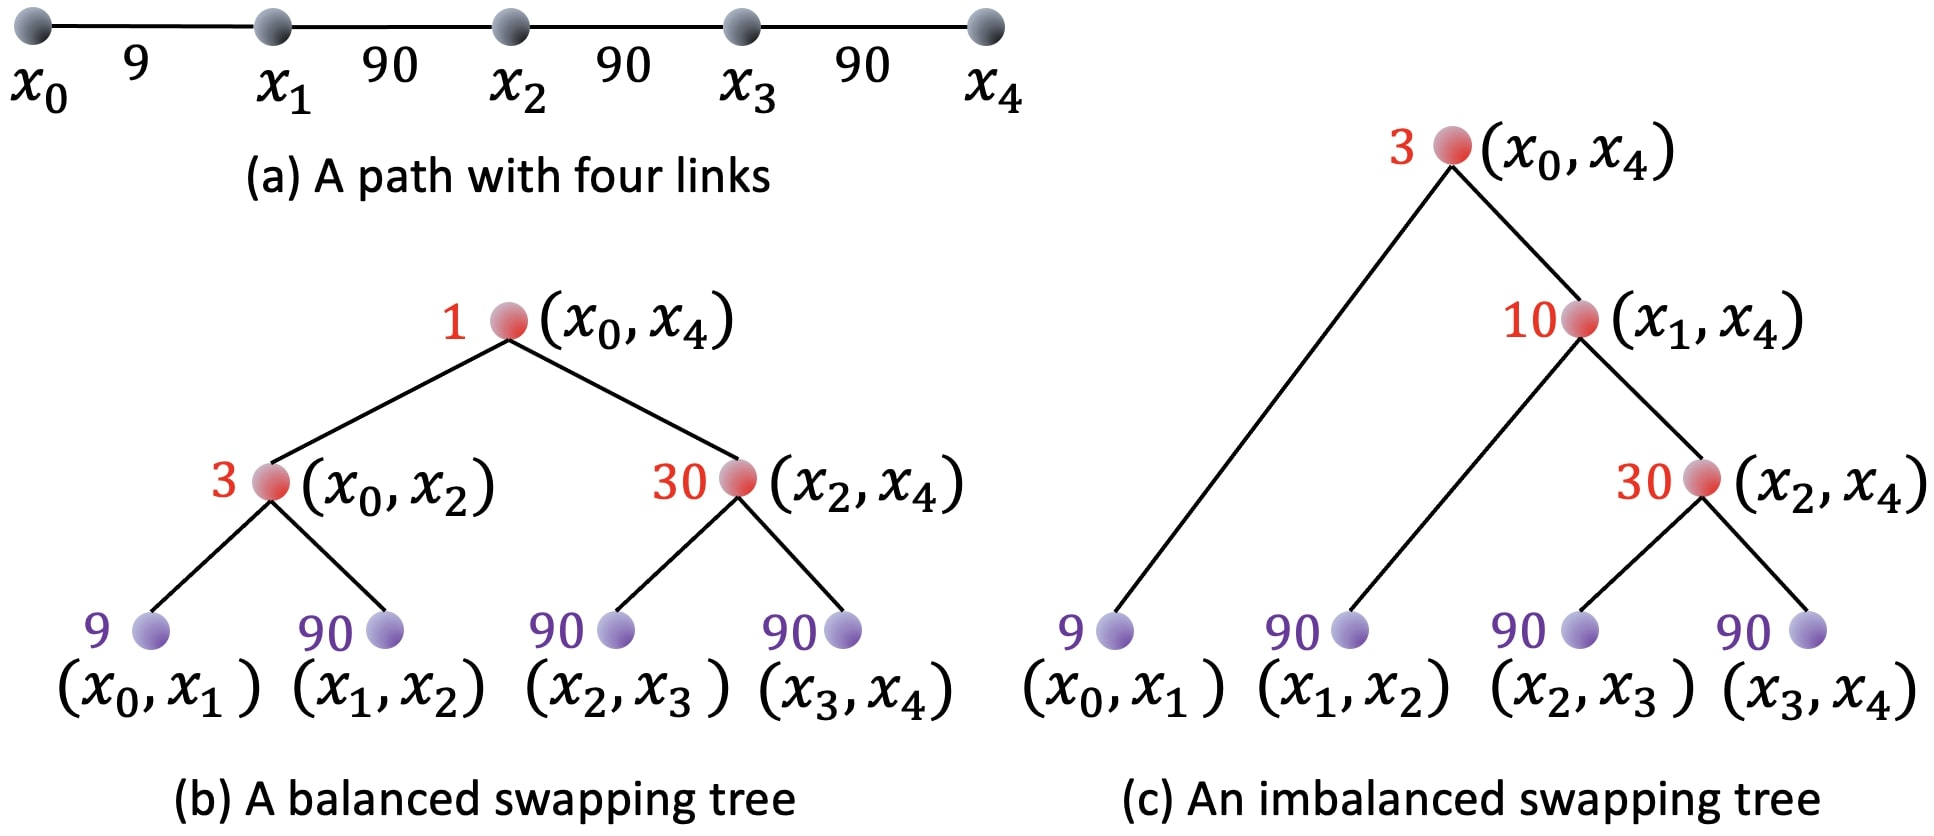
\includegraphics[width=0.8\textwidth]{chapters/swappingtrees/figures/non-balanced-balanced.jpg}
    % \vspace*{0.1in}
    \caption{Consider the path in (a). The imbalanced tree of (b) has a higher \eps generation rate than that of the balanced tree of (c). Here, the numbers represent the \eps generation rates over adjacent links or node-pairs.} 
    % \vspace*{-0.2in}
    \label{fig:swapping_non-balance}
\end{figure}


\softpara{Our Approach (vs.~\cite{caleffi}).}
Though~\cite{caleffi} considers only balanced trees, its 
brute-force algorithm is literally impossible to run for 
networks more than a few tens of nodes.
In our work, we observe that a path has many swapping trees, 
and, in general, imbalanced trees may even
be better; see Figure~\ref{fig:swapping_non-balance}. 
Thus, ~\cite{swapping-tqe-22} design a polynomial-time dynamic programming (DP) algorithm that delivers 
an \textit{optimal} high-fidelity swapping-tree;
the approach effectively considers all possible swapping trees, 
not just balanced ones (note that, even over a single path, 
there are exponentially many trees). 
%Incorporation of fidelity (including decoherence) in our DP approach requires non-trivial observation and analysis (\S\ref{sec:swapping_dec}).
Our \dpalt Heuristic (\S\ref{sec:swapping_efficient}) is closer to~\cite{caleffi}'s work, 
in that both 
consider only balanced trees; however, we use a heuristic metric that facilitates a polynomial-time Dijkstra-like heuristic to select the optimal path, while their recursive metric~\footnote{We note that their formula (Eqn.~10 in~\cite{caleffi}) is incorrect as it either ignores the 3/2 factor or assumes the \eps generations to be synchronized {\bf across all} links. In addition, their expression for "qubit age" ignores the "waiting for \es" time completely. \label{ft:swapping_wrong}} 
(albeit more accurate than ours) is not amenable to an efficient (polynomial-time) search algorithm. 

\para{Other Works.}
In~\cite{Jiang17291}, Jiang et al.\ address a related problem; given a 
path with uniform link-lengths, they give an algorithm for selecting an 
optimal sequence of swapping and purification operations 
to produce an \eps with fidelity constraints.  
In other recent works, Dahlberg et al~\cite{sigcomm19} design physical and link layer protocols
of a quantum network stack, and~\cite{conext20} proposes a data plane protocol to generate \epss
within decoherence thresholds along a \emph{given} routing path. 
More recently, Bugalho et al.~\cite{bugalho2021distributing} propose an algorithm to efficiently distribute multipartite entanglement across over than two nodes.

\eat{
%%%%%%
Most recent works: sigcomm and delft-lp. They both do paths in \os model. 
\cite{sigcomm20} considers the \os model. For the \os model, if we assume a single channel per link, the \eps generation rate for a path (tree doesn't matter) can be
easily derived to be $p^n \bp^n$ per time slot. But, for multiple channels, it requires
a more complex metric -- derived in their paper.
%%%%%%
They use a Dijkstra like algorithm to find an optimal path. Use an iterative procedure
to find paths for more pairs. They use a simplistic model of resource -- multiple channels per link. }

\eat{

; this is clearly infeasible for even networks with 100’s of nodes. (?perhaps not needed?) 

\bleu{The \wt approach has been well analyzed in~\cite{gisin}; they implicitly consider
balanced trees over given paths. More recently,} Caleffi~\cite{caleffi} 
derives an expression\footnote{We note that their formula (Eqn.~10 in~\cite{caleffi}) is incorrect as it either ignores the 3/2 factor, or assumes the \eps generations to be synchronized {\bf across all} links. In addition, their expression for "qubit age" ignores the "waiting for \es" time completely. \label{ft:wrong}} for generation latency of a \textit{balanced} swapping 
tree over a path, and designs
a \bleu{brute-force \textit{exponential}-time algorithm to select an optimal path (by considering all possible simple routes and picking the one with lowest generation latency of the balanced tree).}
}

\eat{
Our dynamic programming approach is very different from~\cite{caleffi};
in effect,~\cite{caleffi} does exhaustive search of all paths, while
our dynamic-programming algorithm (\S\ref{sec:swapping_dp}) effectively considers 
all swapping trees (exponentially many, even
over a single path). 




\eat{Optimality of our approach rests on a non-trivial claim of ensuring disjoint subtrees (Lemma~\ref{lemma:swapping_subtrees}).
%%%%%%%%%%%%%%%%%%%%%%%%%
Incorporating fidelity and decoherence in~\cite{caleffi} is quite straightforward
(though,~\cite{caleffi} incorporates only decoherence; see Footnote~\ref{ft:swapping_wrong});} in contrast, in our dynamic programming approach, incorporation of fidelity (including decoherence) requires non-trivial observation and analysis (\S\ref{sec:swapping_dec}).
%%%%%%%%%%%%%%%%%%%%%
%%%%%%%%%%%%%%%%%%%%%%
Our \dpalt Heuristic (\S\ref{sec:swapping_efficient}) is closer to~\cite{caleffi}'s work, in that both 
consider only balanced trees; however, we use heuristic metric that facilitates a polynomial-time Dijkstra-like heuristic to select the optimal path, while their recursive metric (albeit more accurate
than ours) is not amenable to an efficient (polynomial-time) search algorithm. 
\cb
}